\subsubsection{Testbench và Kết quả mô phỏng Khối điều khiển (Controller)}

\textbf{a. Mô tả kịch bản kiểm chứng (Testbench)} \\
Môi trường mô phỏng khối Controller được thiết lập để kiểm tra chu trình 8 trạng thái (8-Phase) và sự chính xác của các tín hiệu điều khiển đầu ra ứng với từng loại mã lệnh (Opcode). Các kịch bản bao gồm:
\begin{itemize}
    \item \textbf{Khởi tạo và Fetch}: Kiểm tra 4 trạng thái đầu (\texttt{INST\_ADDR} đến \texttt{IDLE}) xem các tín hiệu \texttt{sel}, \texttt{rd}, \texttt{ld\_ir} có bật đúng để nạp lệnh hay không.
    \item \textbf{Lệnh tính toán (ADD/LDA)}: Kiểm tra việc bật tín hiệu \texttt{rd} ở giai đoạn thực thi và tín hiệu \texttt{ld\_ac} ở trạng thái \texttt{STORE}.
    \item \textbf{Lệnh rẽ nhánh (SKZ)}: Kiểm tra tín hiệu \texttt{inc\_pc} có bật thêm ở trạng thái \texttt{ALU\_OP} khi cờ \texttt{is\_zero = 1} hay không.
    \item \textbf{Lệnh nhảy (JMP)}: Kiểm tra tín hiệu \texttt{ld\_pc} có kích hoạt tại trạng thái thực thi để nạp địa chỉ mới.
    \item \textbf{Lệnh lưu trữ (STO)}: Kiểm tra sự phối hợp giữa \texttt{data\_e} và \texttt{wr} để ghi dữ liệu ra bộ nhớ.
\end{itemize}

\textbf{b. Mã nguồn Testbench (Verilog)}
\begin{lstlisting}[language=Verilog, caption={Ma nguon Testbench kiem tra khoi Controller}]
`timescale 1ns / 1ps

module tb_controller();
    // Khai bao cac tin hieu ket noi voi Module Controller
    reg clk;
    reg rst;
    reg [2:0] opcode;
    reg is_zero;
    
    wire sel, rd, ld_ir, halt, inc_pc, ld_ac, ld_pc, wr, data_e;
    wire [2:0] debug_state;

    // Khoi tao Unit Under Test (UUT)
    controller uut (
        .clk(clk), 
        .rst(rst), 
        .opcode(opcode), 
        .is_zero(is_zero),
        .sel(sel), 
        .rd(rd), 
        .ld_ir(ld_ir), 
        .halt(halt), 
        .inc_pc(inc_pc), 
        .ld_ac(ld_ac), 
        .ld_pc(ld_pc), 
        .wr(wr), 
        .data_e(data_e), 
        .debug_state(debug_state)
    );

    // Dinh nghia Opcode giong nhu trong module Controller
    localparam HLT=3'b000, SKZ=3'b001, ADD=3'b010, STO=3'b110, JMP=3'b111;

    // Tao xung clock chu ky 10ns
    always #5 clk = ~clk;

    initial begin
        // --- BUOC 0: Khoi tao he thong ---
        clk = 0; rst = 1; is_zero = 0; opcode = HLT;
        #15 rst = 0; // Tha reset sau 1.5 chu ky clock

        // --- BUOC 1: Kiem tra lenh ADD (Tinh toan) ---
        // Ky vong: ld_ac phai bat o buoc STORE (State 7)
        opcode = ADD; 
        $display("Time=%0t | Bat dau lenh ADD", $time);
        repeat (8) @(posedge clk); 

        // --- BUOC 2: Kiem tra lenh SKZ khi ket qua truoc do bang 0 ---
        // Ky vong: inc_pc phai bat 2 lan (State 6 va State 7)
        opcode = SKZ; is_zero = 1;
        $display("Time=%0t | Bat dau lenh SKZ (Zero=1)", $time);
        repeat (8) @(posedge clk);

        // --- BUOC 3: Kiem tra lenh STO (Ghi bo nho) ---
        // Ky vong: wr va data_e phai bat o buoc STORE (State 7)
        opcode = STO; is_zero = 0;
        $display("Time=%0t | Bat dau lenh STO", $time);
        repeat (8) @(posedge clk);

        // --- BUOC 4: Kiem tra lenh JMP (Nhay dia chi) ---
        // Ky vong: ld_pc phai bat o State 6 va 7
        opcode = JMP;
        $display("Time=%0t | Bat dau lenh JMP", $time);
        repeat (8) @(posedge clk);

        // --- BUOC 5: Kiem tra lenh HLT (Dung he thong) ---
        opcode = HLT;
        $display("Time=%0t | Bat dau lenh HLT", $time);
        repeat (8) @(posedge clk);

        #50;
        $display("Mo phong ket thuc thanh cong!");
        $finish;
    end

    // Tu dong in ket qua ra Console de kiem tra nhanh
    initial begin
        $monitor("T=%4t | State=%d | Op=%b | Halt=%b | IncPC=%b | LdAC=%b | Wr=%b",
        $time, debug_state, opcode, halt, inc_pc, ld_ac, wr);
    end

endmodule
\end{lstlisting}

\textbf{c. Sơ đồ mạch RTL (RTL Schematic)} \\
Sơ đồ tổng hợp khối Controller thể hiện cấu trúc của một máy trạng thái hữu hạn bao gồm bộ đếm trạng thái, bộ giải mã trạng thái kế tiếp và khối logic tổ hợp để tạo ra các tín hiệu điều khiển dựa trên mã lệnh đầu vào.

\begin{figure}[H]
    \centering
    % Thay 'controller_rtl.png' bang ten file anh thuc te cua ban
    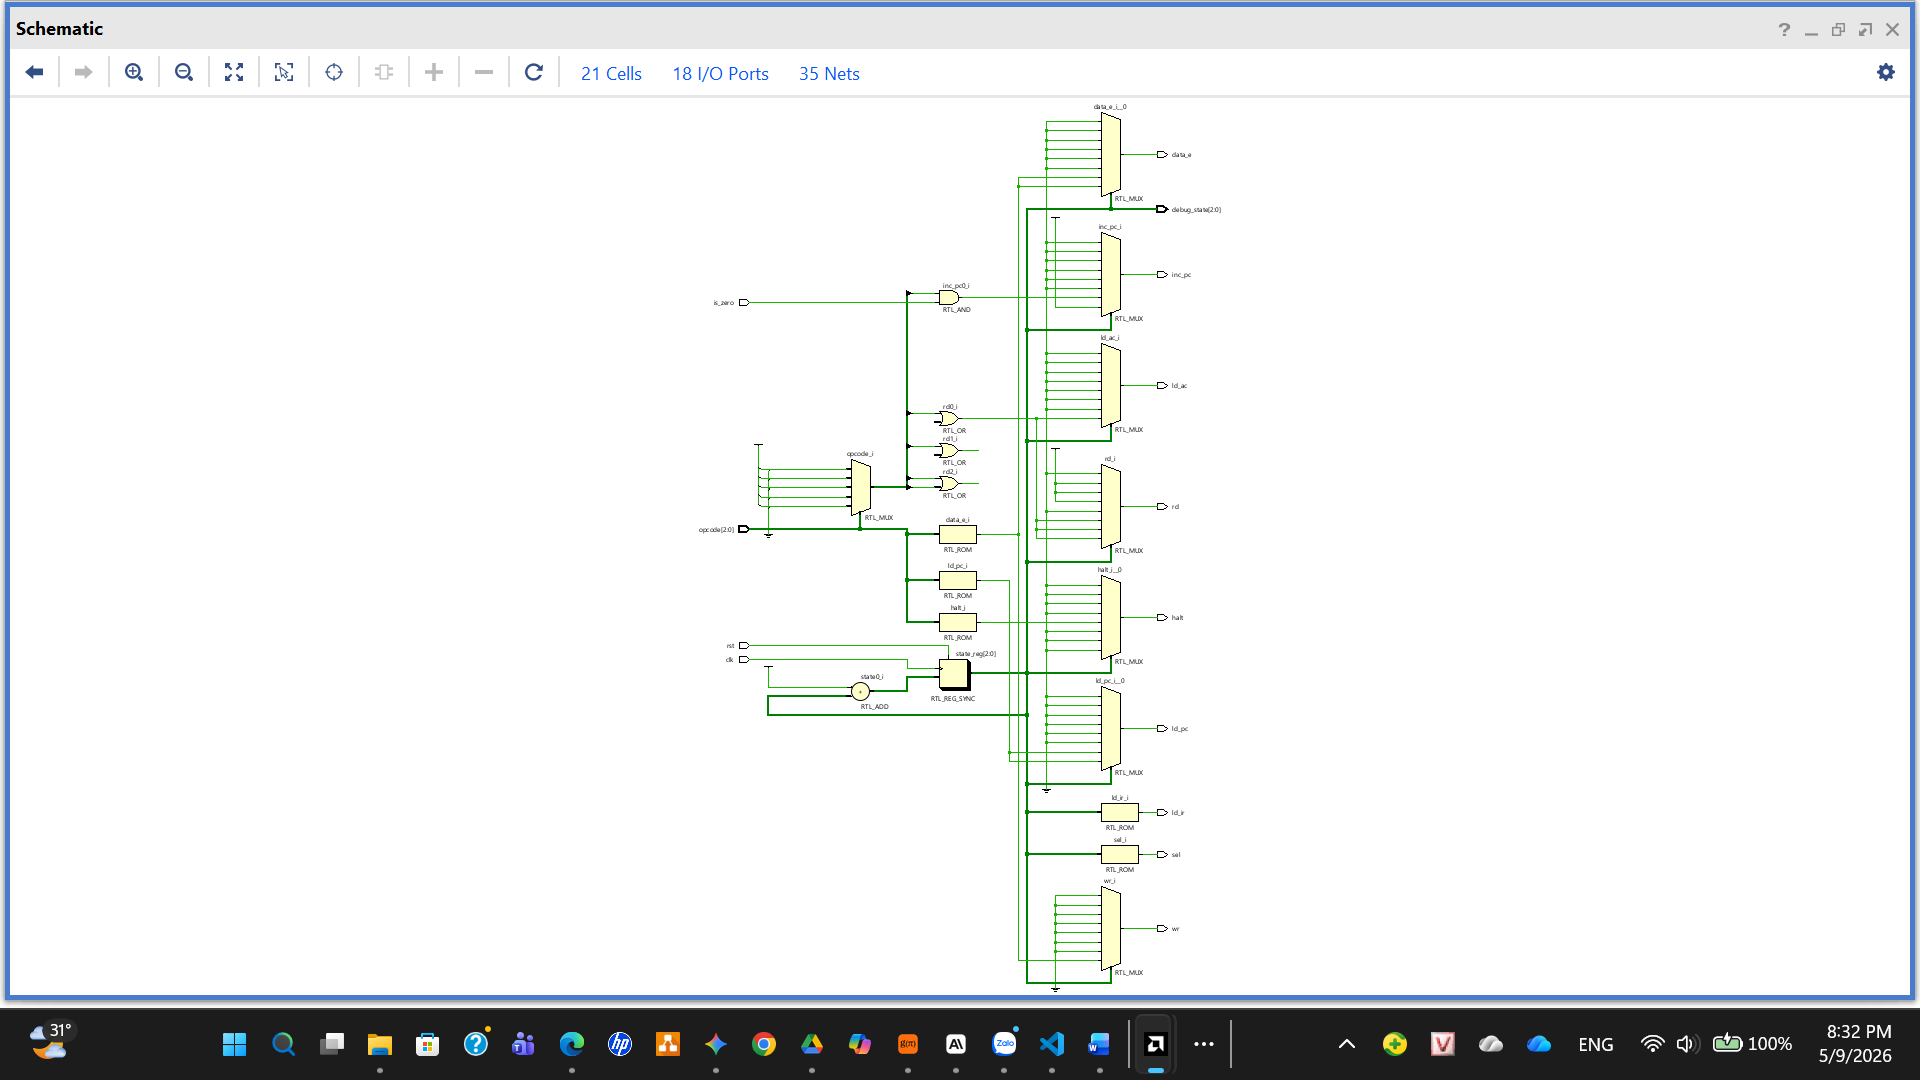
\includegraphics[width=0.9\textwidth]{sodocontrol.png} 
    \caption{Sơ đồ mạch logic (RTL Schematic) của khối Controller}
    \label{fig:ctrl_rtl}
\end{figure}

\textbf{d. Kết quả mô phỏng (Waveform)} \\
Quá trình chuyển đổi trạng thái và phản hồi của các tín hiệu điều khiển được ghi lại chi tiết trên giản đồ thời gian.

\begin{figure}[H]
    \centering
    % Thay 'controller_waveform.png' bang ten file anh thuc te cua ban
    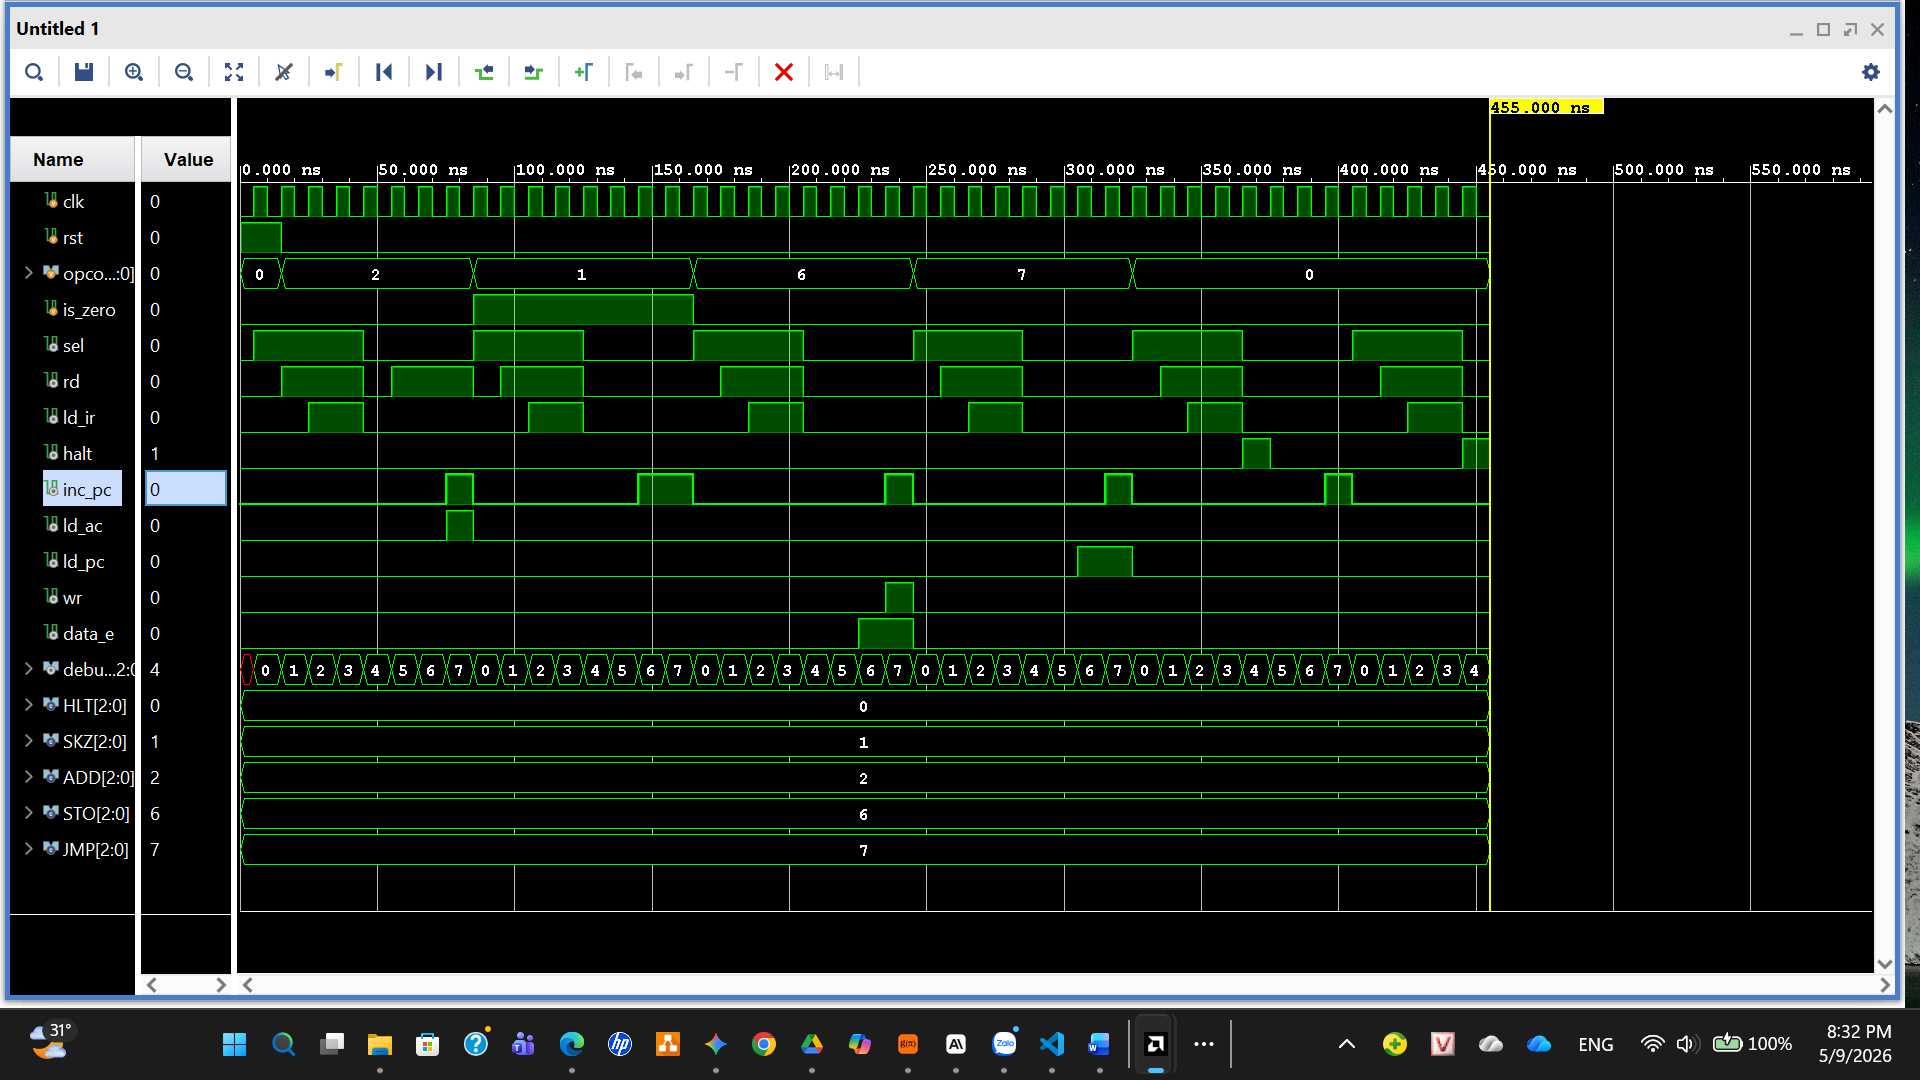
\includegraphics[width=\textwidth]{wavecontroller.png} 
    \caption{Giản đồ thời gian (Waveform) mô phỏng khối Controller}
    \label{fig:ctrl_wave}
\end{figure}

\textbf{e. Kết quả xuất ra màn hình (Console Output)} 
\begin{figure}[H]
    \centering
    % Thay 'controller_console.png' bang ten file anh thuc te cua ban
    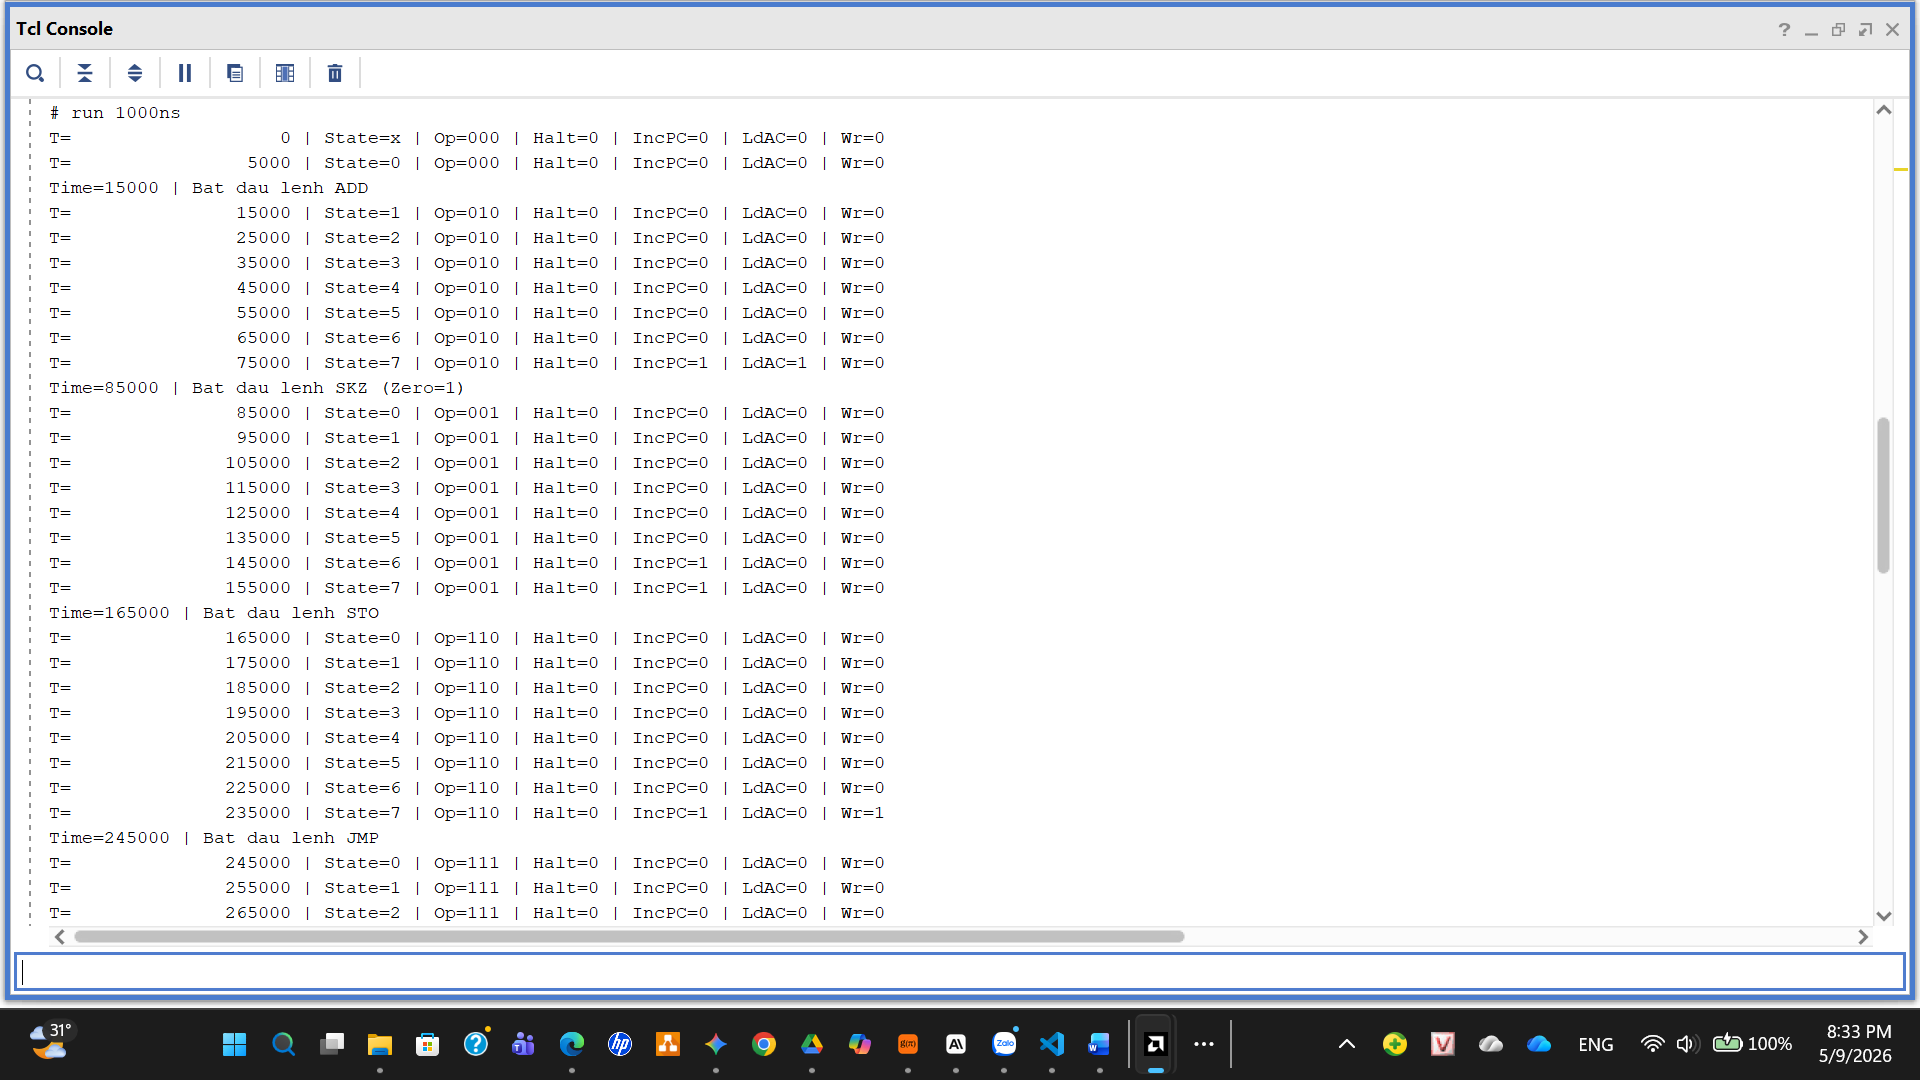
\includegraphics[width=0.8\textwidth]{1.png} 
    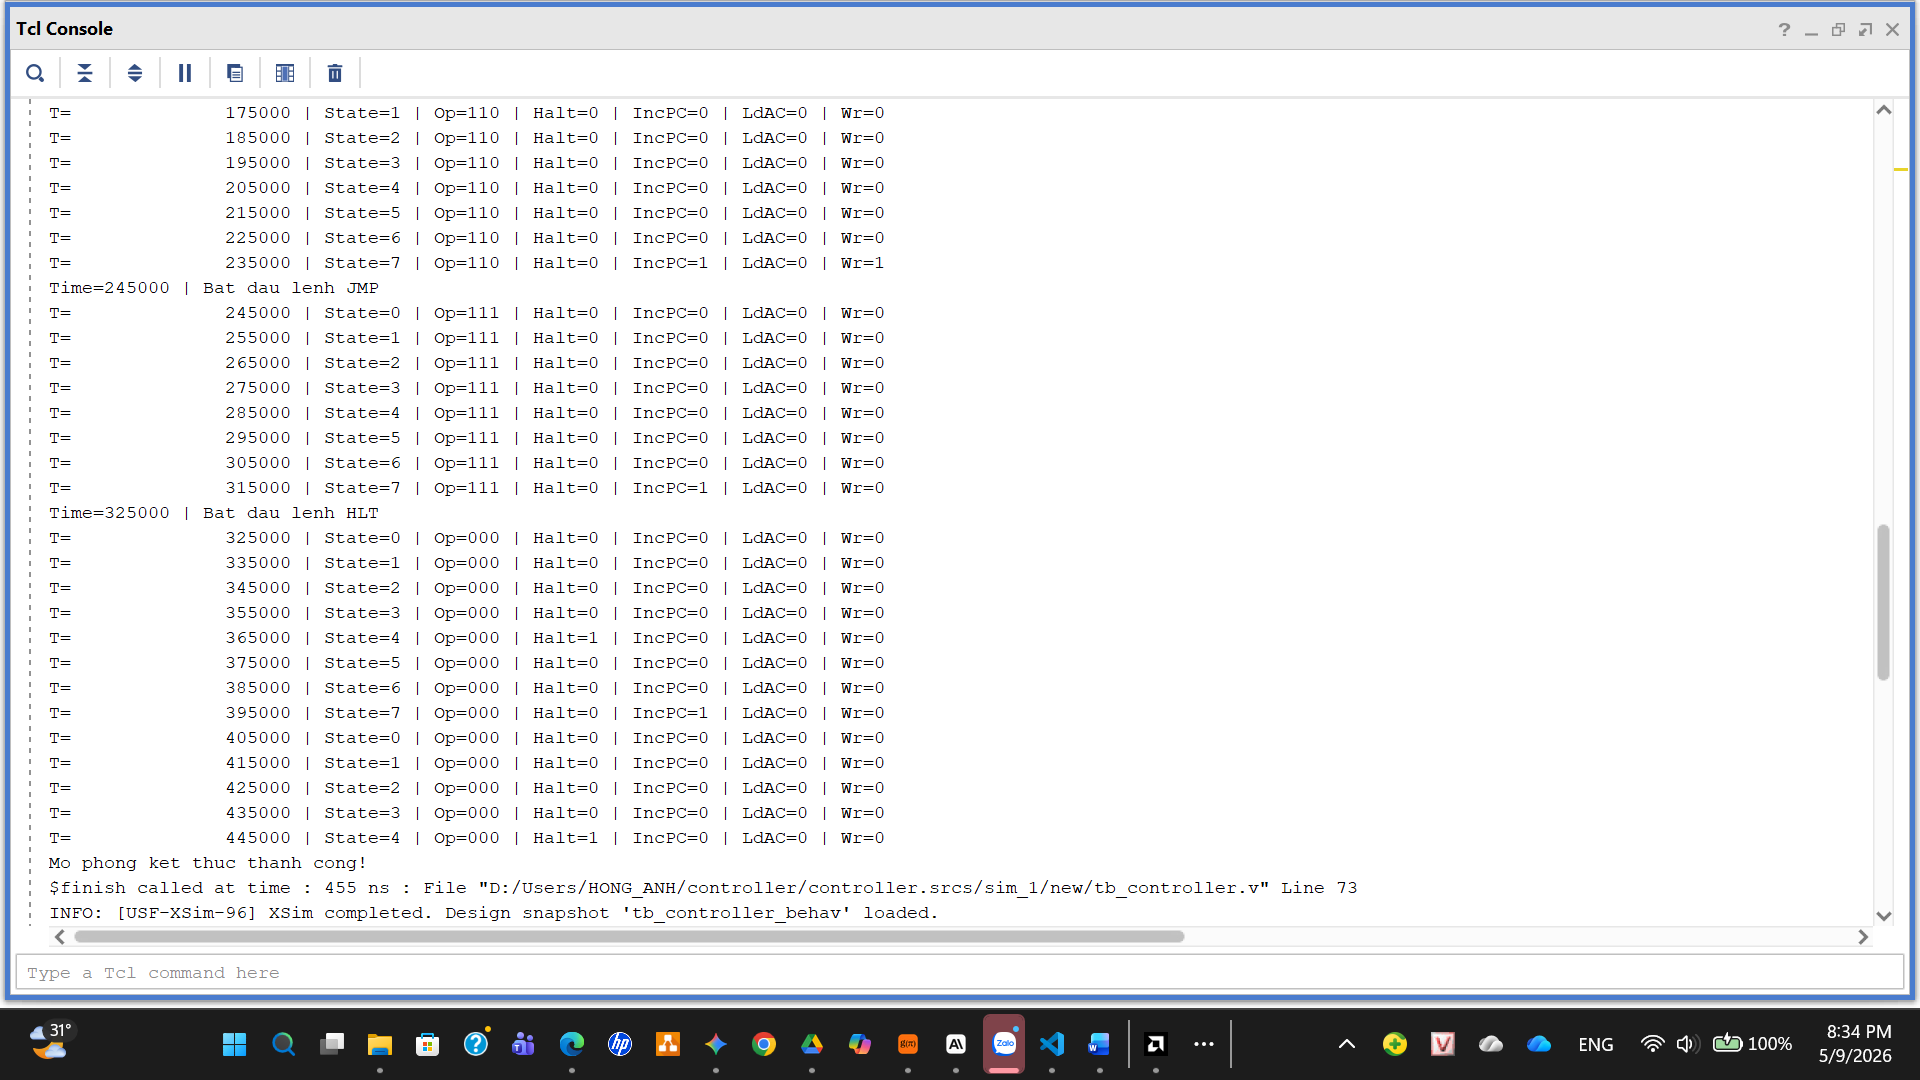
\includegraphics[width=0.8\textwidth]{2.png} 
    \caption{Kết quả Console mô phỏng khối Controller}
    \label{fig:ctrl_console}
\end{figure}

\textbf{Đánh giá kết quả:}
\begin{itemize}
    \item \textbf{Tính tuần tự}: Tín hiệu \texttt{debug\_state} thay đổi liên tục từ 0 đến 7, đảm bảo chu trình 8 bước không bị gián đoạn.
    \item \textbf{Đúng đắn về logic}: Tín hiệu \texttt{inc\_pc} luôn bật ở trạng thái \texttt{STORE} cho mọi lệnh, riêng với lệnh \texttt{SKZ} khi cờ \texttt{is\_zero = 1}, nó còn bật thêm ở trạng thái \texttt{ALU\_OP}, giúp nhảy qua lệnh kế tiếp chính xác như thiết kế.
    \item \textbf{Cơ chế nạp/ghi}: Tín hiệu \texttt{ld\_ac} (cho lệnh tính toán) và \texttt{wr} (cho lệnh ghi) chỉ xuất hiện ở bước cuối cùng, đảm bảo tính ổn định của dữ liệu trên Bus hệ thống trước khi thực hiện thao tác lưu trữ.
\end{itemize}